\documentclass[12pt,letterpaper,oneside]{report}
%Puedes verificar todas las especificaciones de este documento en thesis.sty
\usepackage{thesis}
  
  
\usepackage{atbegshi}
\AtBeginDocument{\AtBeginShipoutNext{\AtBeginShipoutDiscard}}




\begin{document}

\begin{titlepage}

\setlength{\voffset}{-0.5cm}
\setlength{\hoffset}{0.9cm}
\setlength{\headsep}{0pt}
\setlength{\headheight}{0pt}
\setlength{\oddsidemargin}{-0.8in}
\setlength{\marginparwidth}{-0.5cm}
\setlength{\textwidth}{15cm}
\setlength{\footskip}{2pt}
\setlength{\topmargin}{0in}
\setlength{\textheight}{27cm}
\setlength{\fboxrule}{3pt}


\begin{tabular}{p{2.4cm}p{14cm}}

\includegraphics[width=2.4cm]{IPN LOGO.png}
\begin{center}
\rule[2cm]{0.8mm}{15cm}%vertical
\hspace{1pt}
\rule[2cm]{0.4mm}{15cm}%vertical
\vspace{-2cm}

\includegraphics[width=2.5cm]{ESE LOGO.png}

\end{center}
&
\vspace{-3.5cm}
\begin{center}
\rule[1mm]{15cm}{0.4mm}%horizontal
\vspace{0.1pt}
\rule[3mm]{15cm}{0.8mm}%horizontal
\\
\LARGE{\bf{INSTITUTO POLITÉCNICO NACIONAL}}\\
\vspace*{0.3cm}
\Large{\bf{ESCUELA SUPERIOR DE ECONOMÍA}}\\
\vspace*{0.3cm}
\large{\bf{Sección de Estudios de Posgrado e Investigación}}

\vspace{2\baselineskip}
{\Large \bf{Manzanas estocásticas:}}\\
\vspace*{0.2cm}
{\Large \bf{una aplicación con Machine Learning}}\\
%\vspace*{0.2cm}
%\Large \bf{va aquí}\\
\vspace*{1.6cm}
\LARGE{\bf T E S I S}

\vspace*{1.2cm}
{\large QUE PARA OBTENER EL GRADO DE}\\
\vspace*{0.4cm}
{\large \bf{MAESTRO EN CIENCIAS ECONÓMICAS}\\
\vspace*{-0.1cm}
{\large \bf{(Economía Financiera)}\\
\vspace*{0.7cm}
{\large \bf{Presenta:}}


\vspace*{1cm}
{\large \bf{Tu nombre}}\\


\vspace*{3cm}

\small CDMX, MÉXICO. \hspace{4cm} FEBRERO DE 2023.
\end{center}
\end{tabular}

% \newpage

\end{titlepage}

\normalsize


%AGREGA CAPÍTULOS E ÍNDICE



\pagenumbering{roman}
\normalsize

\chapter*{\centerline{AGRADECIMIENTOS}}\label{chapter:agradecimientos}
%\setcounter{page}{0}
\pagenumbering{roman}
Escribe tus agradecimientos...
\pagebreak

\phantomsection
\setcounter{tocdepth}{2}    % Sets maximum depth of Table Of Contents
\renewcommand{\contentsname}{INDICE}
\tableofcontents

\renewcommand{\listfigurename}{ÍNDICE DE FIGURAS}
\renewcommand{\listtablename}{ÍNDICE DE TABLAS}

\clearpage \phantomsection
\addcontentsline{toc}{chapter}{\listfigurename}
\listoffigures
\pagebreak


\clearpage \phantomsection
\addcontentsline{toc}{chapter}{\listtablename}
\listoftables
\pagebreak


\addcontentsline{toc}{chapter}{GLOSARIO}
\chapter*{\centerline{GLOSARIO}}\label{chapter:GLOSARIO}
\textbf{Inflación}:  Aumento generalizado y sostenido de los precios de bienes y servicios en un país.
\textbf{Inflación subyacente}:  Aumento de los precios del subconjunto del INPC, que contiene a los genéricos con cotizaciones menos volátiles o con evolución más estable.



\pagebreak



\addcontentsline{toc}{chapter}{ABREVIACIONES}
\chapter*{\centerline{ABREVIACIONES}}\label{chapter:ABREVIACIONES}
%\setcounter{page}{0}
%\renewcommand{\thechapter}{\roman{chapter}}
\begin{tabular}{ll}
\textbf{INPC} & Índice Nacional de Precios al Consumidor \\
\textbf{IPC}  & Índice de Precios y Cotizaciones \\
\textbf{PIB}  & Producto Interno Bruto \\
\end{tabular}

\pagebreak

\addcontentsline{toc}{chapter}{RESUMEN}
\chapter*{\centerline{RESUMEN}}\label{chapter:RESUMEN}
%\setcounter{page}{0}
%\renewcommand{\thechapter}{\roman{chapter}}
La presente investigación tiene por objetivo...

\textit{Palabras clave:} palabra clave 1, palabra clave 2, palabra clave 3.
\pagebreak

\addcontentsline{toc}{chapter}{ABSTRACT}
\chapter*{\centerline{ABSTRACT}}\label{chapter:Abstract}
%\setcounter{page}{0}
%\renewcommand{\thechapter}{\roman{chapter}}
The aim of this research is...

\textit{Keywords:} keyword 1, keyword 2, keyword 3.
\pagebreak

\addcontentsline{toc}{chapter}{INTRODUCCIÓN}
\chapter*{INTRODUCCIÓN}\label{chapter:Introducción}
%\onehalfspacing
\setcounter{page}{0}
\pagenumbering{arabic}
Escribe tu introducción.
\pagebreak


\addcontentsline{toc}{chapter}{CAPÍTULO 1. AÑADE CAPÍTULOS Y SUBCAPÍTULOS}
\chapter*{CAPÍTULO 1. CAPÍTULOS Y SUBCAPÍTULOS}\label{chapter:Capítulo1}
\onehalfspacing
%\setcounter{page}{0}
%\pagenumbering{arabic}
\setstretch{2}
%\setlength{\parindent}{3em}
\setlength{\parskip}{1em}

Escribe tu capítulo 1


\section{Añade tu primer apartado}
\setlength{\parindent}{0em}

\section{Añade tu segundo apartado}
\setlength{\parindent}{0em}

Agrega notas al pie de página\footnote{También puedes agregar url de páginas de internet, por ejemplo: \url{http://www.youtube.com/c/AnaMetriks}}.

\setlength{\parindent}{2em}
Escribe tu siguiente párrafo con sangría.



\subsection{Añade más subapartados}
\setlength{\parindent}{0em}

\section{Añade el tercero apartado}
\setlength{\parindent}{0em}

\addcontentsline{toc}{chapter}{CAPÍTULO 2. AÑADE ECUACIONES, FIGURAS Y TABLAS}
\chapter*{CAPÍTULO 2. ECUACIONES, FIGURAS Y TABLAS}\label{chapter:Capítulo2}
\setcounter{chapter}{2}
\setcounter{section}{0}
\onehalfspacing
%\setcounter{page}{0}
%\pagenumbering{arabic}
\setstretch{2}
%\setlength{\parindent}{3em}
\setlength{\parskip}{1em}

Escribe tu capítulo 2


\section{Añadamos algunas ecuaciones}
\setlength{\parindent}{0em}

Enumera tus ecuaciones

Regresión Lineal (Mínimos Cuadrados Ordinarios)

\begin{equation}
\hat{\beta }=min\sum_{i=1}^{n}\left ( y_i-\beta_0-\sum_{i=1}^{p} \beta _{j}x_{ij} \right )^{2}
\end{equation}

O si quieres no las enumeres

$$\hat{\beta }=min\sum_{i=1}^{n}\left ( y_i-\beta_0-\sum_{i=1}^{p} \beta _{j}x_{ij} \right )^{2}$$

O puedes utilizar tus ecuaciones dentro del texto $\hat{\beta }=min\sum_{i=1}^{n}\left ( y_i-\beta_0-\sum_{i=1}^{p} \beta _{j}x_{ij} \right )^{2}$.

Y si tienes ecuaciones muy largas, las puedes hacer utilizando:

\begin{equation}
\begin{aligned}
Y  = & [\alpha_0+\alpha_1\ (Y-T)-\alpha_2\ R]+[\beta_0+\beta_1 Y-\beta_2 R]+G\\
Y  = & [\alpha_0+\alpha_1\ Y-\alpha_1\ [\gamma_0+\gamma_1\ Y]-\alpha_2 R]+[\beta_0+\beta_1 Y-\beta_2R]+G\\
Y  = &  [\alpha_0+\alpha_1\ \gamma_0+\beta_0\ ]+[\alpha_1-\alpha_1 \gamma_1+\beta_1 ]Y-[\alpha_2+\beta_2]R+G\\
Y  = & \alpha_1-\alpha_1\ \gamma_1+\beta_1\ ]Y=[\alpha_0+\alpha_1 \gamma_0+\beta_0 ]-[\alpha_2+\beta_2 ]R+G\\
Y  = & [1/(1-\alpha_1+\alpha_1\ \gamma_1-\beta_1\ )][(\alpha_0-\alpha_1 \gamma_0+\beta_0)-(\alpha_2+\beta_2)R+G] 
\end{aligned}
\end{equation}

\section{Añadamos unas figuras}


\begin{figure}[h!]
\caption{Pronóstico de crecimiento económico global 2020}
\label{fig:GrowthGDP}
\centering
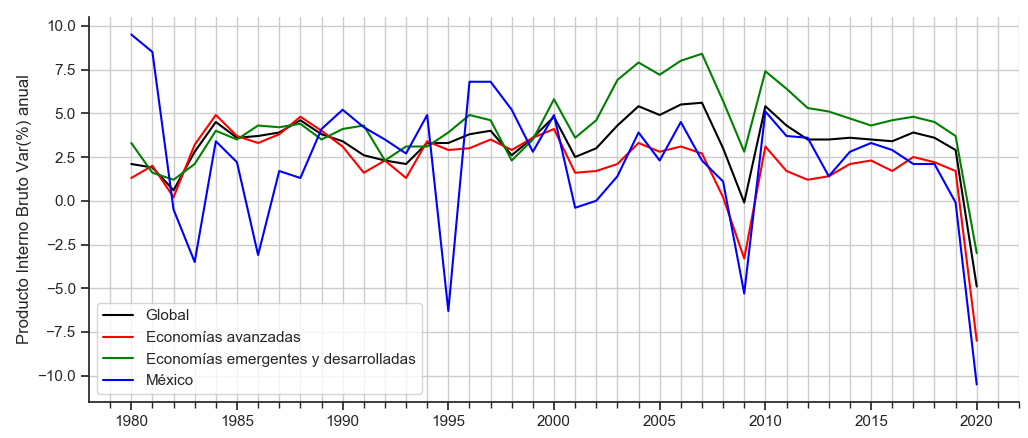
\includegraphics[width=1\textwidth]{Figuras/GDP.png}
\caption*{Fuente: elaboración propia con datos del FMI}
\end{figure}

\newpage
\section{También una tabla}

\begin{table}[h]
\centering
\caption{Comparación de contracciones económicas}
\begin{tabular}{ccccc}
\textbf{Año} &
  \textbf{Mundial} &
  \textbf{\begin{tabular}[c]{@{}c@{}}Economías\\ avanzadas\end{tabular}} &
  \textbf{\begin{tabular}[c]{@{}c@{}}Economías emergentes\\ y desarrolladas\end{tabular}} &
  \textbf{México} \\ \hline
1995     & 3.3  & 2.9  & 3.9  & -6.3  \\
2009     & -0.1 & -3.3 & 2.8  & -5.3  \\
$2020^E$ & -4.9 & -8.0 & -3.0 & -10.5 \\ \hline
\end{tabular}
\begin{tablenotes}
\centering
\item Fuente: elaboración propia con datos del FMI.
\end{tablenotes}
\end{table}

Aquí podemos describir los resultados de la tabla.

\begin{table}[h]
\centering
\caption{Precios de OMA}
\label{tab:OMA}
\begin{tabular}{ll}
\multicolumn{1}{c}{\textbf{Date}} & \multicolumn{1}{c}{\textbf{Close}} \\ \hline
15/04/2016                        & 100.169998                         \\
18/04/2016                        & 99.339996                          \\
19/04/2016                        & 100.699997                         \\
20/04/2016                        & 100.68                             \\
21/04/2016                        & 100.080002                         \\
22/04/2016                        & 101.660004                         \\
25/04/2016                        & 101.690002                         \\
26/04/2016                        & 97.059998                          \\
27/04/2016                        & 99.639999                         
\end{tabular}
\begin{tablenotes}
\centering
\item Fuente: elaboración propia con datos del Yahoo Finance.
\end{tablenotes}
\end{table}


\addcontentsline{toc}{chapter}{CAPÍTULO 3. CITAR CORRECTAMENTE}
\chapter*{CAPÍTULO 3. CITAR CORRECTAMENTE}\label{chapter:Capítulo3}
\setcounter{chapter}{3}
\setcounter{section}{0}
\onehalfspacing
%\setcounter{page}{0}
%\pagenumbering{arabic}
\setstretch{2}
%\setlength{\parindent}{3em}
\setlength{\parskip}{1em}

\section{Incorporación de citas}

Incorpora las citas, ya sea que cite una idea dentro del texto, por ejemplo.

El uso de \textit{Machine Learning} ha revolucinado la forma en como se hace valuación financiera \parencite{Moat}.

O bien, se puede citar como:

De acuerdo con \textcite{Moat}, el uso de \textit{Machine Learning} ha revolucinado la forma en como se hace valuación financiera.

\section{Incorporación de viñetas}

Finalmente, puedes crear \textit{bullets} o viñetas utilizando el comando "\textit{itemize}".

\begin{itemize}
    \item Primera viñeta
    \item Segunda viñeta
\end{itemize}

O bien, puedes enumerar con el comando "\textit{enumerate}"

\begin{enumerate}
    \item Primera viñeta
    \item Segunda viñeta
\end{enumerate}


\addcontentsline{toc}{chapter}{CONCLUSIONES}
\chapter*{CONCLUSIONES}\label{chapter:Conclusiones}
%\setcounter{page}{0}
\setstretch{2}
%\setlength{\parindent}{3em}
\setlength{\parskip}{1em}

Menciona los principales hallazgos de tu investigación.





%\chapter*{REFERENCIAS}
\printbibliography[title={REFERENCIAS}]
\addcontentsline{toc}{chapter}{REFERENCIAS}
%\chapter*{\centerline{REFERENCIAS}}\label{chapter:referencias}

%\input{Referencias}
%\bibliographystyle{}

\pagebreak
\end{document} 